\documentclass[runningheads]{llncs}
\usepackage[newfloat]{minted}
\setminted[cpp]{
frame=lines,
linenos,
breaklines,
fontsize=\footnotesize,
framesep=2mm
}
\usepackage{caption}
\usepackage{graphicx}
\usepackage[portuguese]{babel}
\usepackage{hyphenat}
\usepackage{lscape}
\usepackage{microtype} % melhora a formatação do texto para evitar overfull box, entre outros
\usepackage{hyperref}
\usepackage{amsmath}
\usepackage{subfiles}
% to insert sourcecode
\newenvironment{code}{\captionsetup{type=listing}}{}
\SetupFloatingEnvironment{listing}{name=\underline{\textbf{CGDraw} Source Code}}

\begin{document}
%
\title{Relatório Computação Grafica - Fase 3}
\author{Marco Sousa\inst{1,2}\orcidID{62608} \and
    José Malheiro\inst{1,2}\orcidID{93271} \and
    Miguel Fernandes\inst{1,2}\orcidID{94269}}
%
\institute{Universidade do Minho\\
    \and Licenciatura em Engenharia Informática, Braga, Portugal}
%
\maketitle              % typeset the header of the contribution
%
\begin{abstract}
    Com a construção do esqueleto da cena principal, em conjunto com as animações
    dos elementos integrantes, o próximo passo seria a população do modelo
    com texturas e iluminação.
    No caso das texturas, para cada umas das figuras geométricas deve ser 
    calculadas as respetivas coordenadas para mapear a imagem no objeto,
    utilizando os conceitos de \textit{mipmapping}(\textit{Nearest, on the lef} 
    \& \textit{Linear, on the right}).
    Na tentativa de definir a iluminação, todas as normais de cada objeto devem 
    ser calculadas.

    Deste modo, o modelo do \textbf{sistema solar} será alterado 
    para incluir estas alterações e produzir a maquete final.
    
    \keywords{ OpenGL \and GLUT \and Figuras Geométricas \and 3D \and C++ \and Texturas \and Iluminação \and Normais \and Coordenadas de Textura}
    \end{abstract}
    %
    %
    %
    \section{Introdução}
    \subsection{Contextualização}
    No seguimento da fase III do projeto da disciplina de Computação Gráfica 
    da Licenciatura em Engenharia Informática da Universidade do Minho, 
    foi proposta, numa última fase, a implementação de texturas e iluminação no projeto,
    através do cálculo das \textbf{coordenadas de textura} e \textbf{normais}
    a cada figura geométrica. 
    Tudo irá culminar na atualização do modelo do sistema solar
    previamente construído com estes parâmetros.
    
    \subsection{Breve Descrição do Enunciado Proposto}
    
    O cerne da última fase (IV) do projeto implica alterações ao nível do \textit{generator} e do \textit{engine} previamente definidos.
    Deste modo, pretende-se:
    \begin{itemize}
        \item [\textit{generator}]
            {Calcular as normais e coordenadas de textura para 
            \textbf{cada vértice} das figuras geométricas.}
        \item [\textit{engine}]
            {Ativar as funcionalidades de iluminação e 
            texturização, utilizando as normais e coordenadas
            de textura definidas.}
    \end{itemize}
    
    No que toca ao \textit{generator}, os novos ficheiros \textit{.3D} 
    devem ser alterados para incluir os vetores \textbf{normais} e 
    as coordenadas de \textbf{textura} da respetiva figura geométrica.
    Deste modo, serão incluidas as \textit{tags}:
    \begin{itemize}
        \item[\textit{normals}]{Todos os vetores normais da figura geométrica.}
        \item[\textit{texture}]{Todas as coordenadas de textura da figura geométrica.} 
    \end{itemize}

    Relativamente à \textit{engine}, devem ser criadas e implementadas
    as \textbf{cores} e texturas de cada figura geométrica permitida.
    Adicionalmente, será necessário definir a(s) luz(es) (tipo e parâmetros) 
    para a cena principal.
    Deste modo, para cada modelo (\textit{model}) do ficheiro \textit{.XML} a ler, 
    encontram-se as \textit{tags}:
    \begin{enumerate}
        \item[\textit{texture}]{Inclui o \textit{path} para a textura, no atributo \textit{file}, 
                                a ser aplicada na figura geométrica.}
        \item[\textit{color}]{Para cada figura geométrica devem ser definidos os componentes:}
        \begin{enumerate}
            \item[\textit{diffuse}]{Cor \textbf{difusa} do objeto - (Em \textit{RGB}).}
            \item[\textit{ambient}]{Cor \textbf{ambiente} do objeto - (Em \textit{RGB}).}
            \item[\textit{specular}]{Cor \textbf{especular} do objeto - (Em \textit{RGB}).}
            \item[\textit{emissive}]{Cor \textbf{emissiva} do objeto - (Em \textit{RGB}).}
            \item[\textit{shininess}]{Valor da refletividade da luz no objeto.}
        \end{enumerate}
    \end{enumerate}
    \dots sendo necessário utilizar as coordenadas de textura 
    calculadas no generator para desenhar a imagem no objeto.

    Para cada cena podem ser definidas a origem para uma ou mais luzes, 
    do tipo:
    \begin{itemize}
        \item[\textit{point}]{Especificada a posição da luz.}
        \item[\textit{directional}]{Epecificada a direção da luz.}
        \item[\textit{spotlight}]{Epecificadas a posição e direção das luzes,
                                  bem como o ângulo \textit{cutoff}.}
    \end{itemize}

    A partir destas alterações apresentar todo o sistema solar como um modelo texturizado e iluminado, 
    obedecendo à estrutura previamente definida para a cena principal.
    
    \section{Trabalho Realizado}
    
    Funcionalidades Implementadas:
    
    \begin{enumerate}
        \item \textit{Generator}
        \begin{enumerate}
            \item Gerar as normais para cada vértice das figuras geométricas. (\ref{subsec:normals})
            \item Gerar as coordenadas de textura para cada figura geométrica. (\ref{subsec:texCoord})
            \item Atualização do ficheiro \textit{.3D}, com as \textit{tags} 
                  \textit{normals} e \textit{texture}.(\ref{subsec:writer})
            \begin{enumerate}
                \item[\textit{ADICIONAL}]{Criação de um círculo de asteróides.} (\ref{subsec:aster})
            \end{enumerate}
        \end{enumerate}
        \item \textit{Engine}
        \begin{enumerate}
            \item Implementação da iluminação:
            \begin{enumerate}
                \item num \textit{point}, através da sua posição.
                \item \textit{directional}, através da direção do foco.
                \item de um \textit{spotlight}, através da posição, direção 
            \end{enumerate}
            \item Implementação de texturas, a partir do \textit{path} da imagem a inserir.
            \item Implementação das cores difusa, ambiente, especular, emissiva e o coeficiente
                  de \textit{shininess} do objeto.
        \end{enumerate}
        \item Sistema Solar 
        \begin{enumerate}
            \item Transição para um modelo iluminado e texturizado.
            \item Adição do cinturão de asteroides.
        \end{enumerate}
    \end{enumerate}
    
    \subfile{generator.tex}
    \subfile{engine.tex}
    \subfile{solar_system.tex}

    \subsection{Testes realizados}
    Para avaliar o desenvolvimento do projeto foram testados os ficheiros de testes disponiblizados
    pela equipa docente e comparou-se com as imagens com o resultado. As seguintes imagens compararam
    o modelo desenvolvido pelo grupo(lado esquerdo) com as imagens disponiblizadas.

    \begin{landscape}
        \begin{figure}
            \centering
            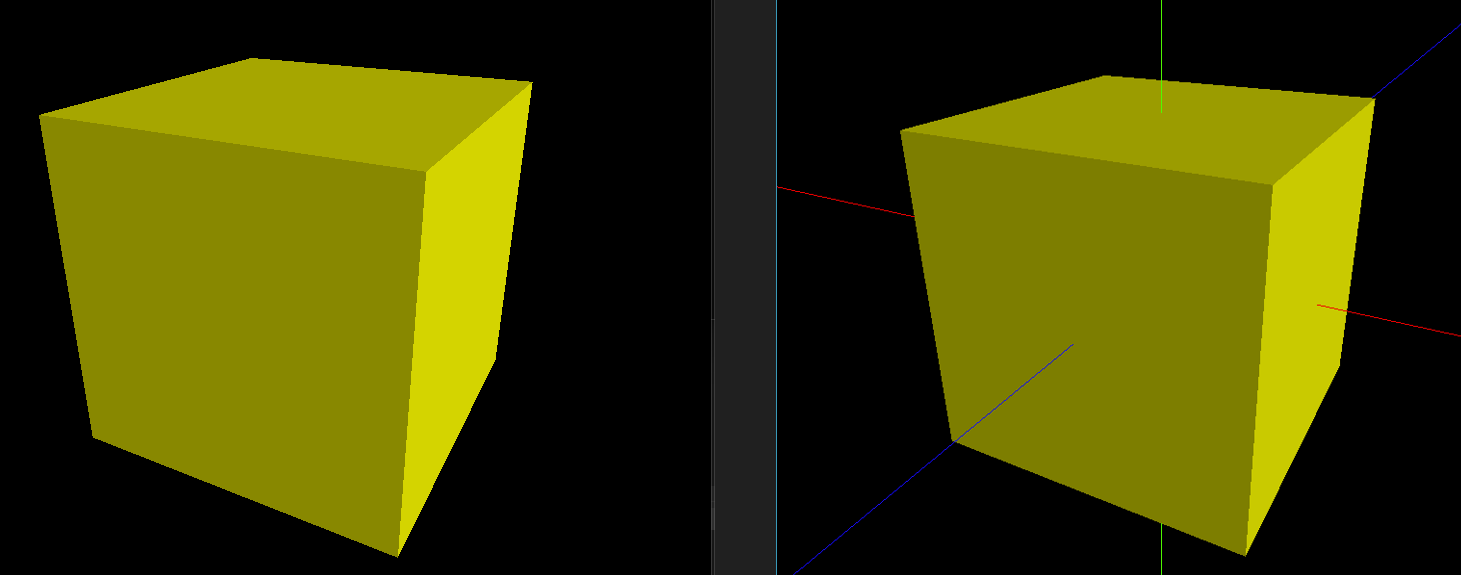
\includegraphics[width=\linewidth]{assets/testes/teste_4_1.png}
            \caption{Resultado do \textit{test_4_1}} \label{fig:teste_4_1}
        \end{figure}
    \end{landscape}

    \begin{landscape}
        \begin{figure}
            \centering
            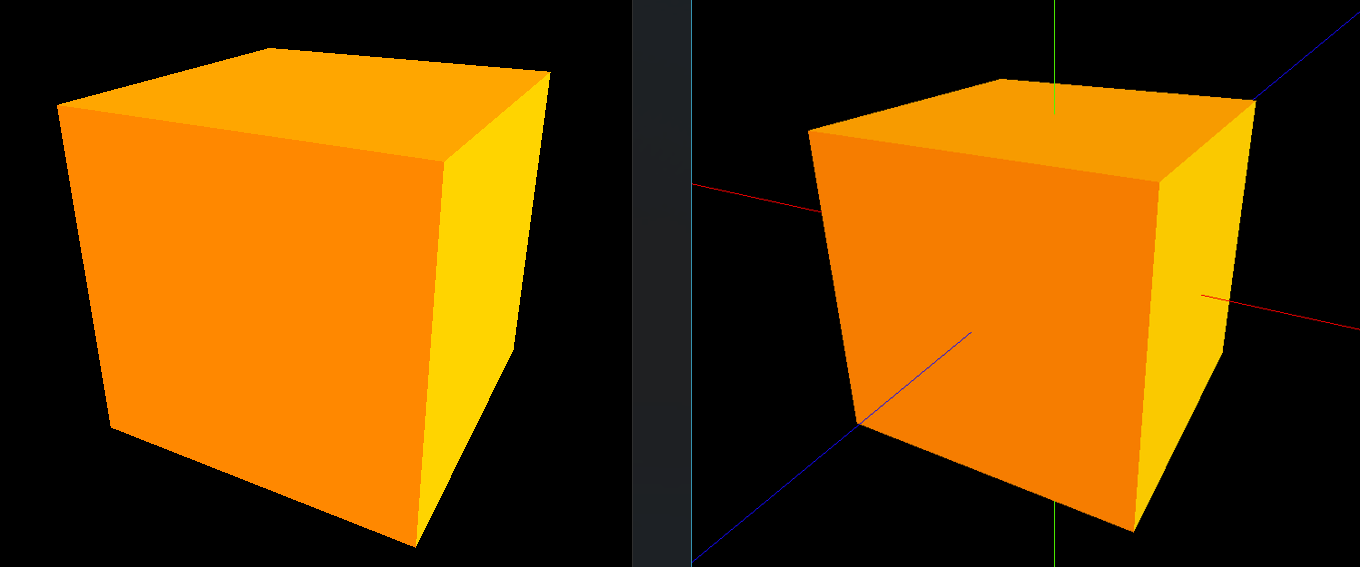
\includegraphics[width=\linewidth]{assets/testes/teste_4_2.png}
            \caption{Resultado do \textit{test_4_2}} \label{fig:teste_4_2}
        \end{figure}
    \end{landscape}

    \begin{landscape}
        \begin{figure}
            \centering
            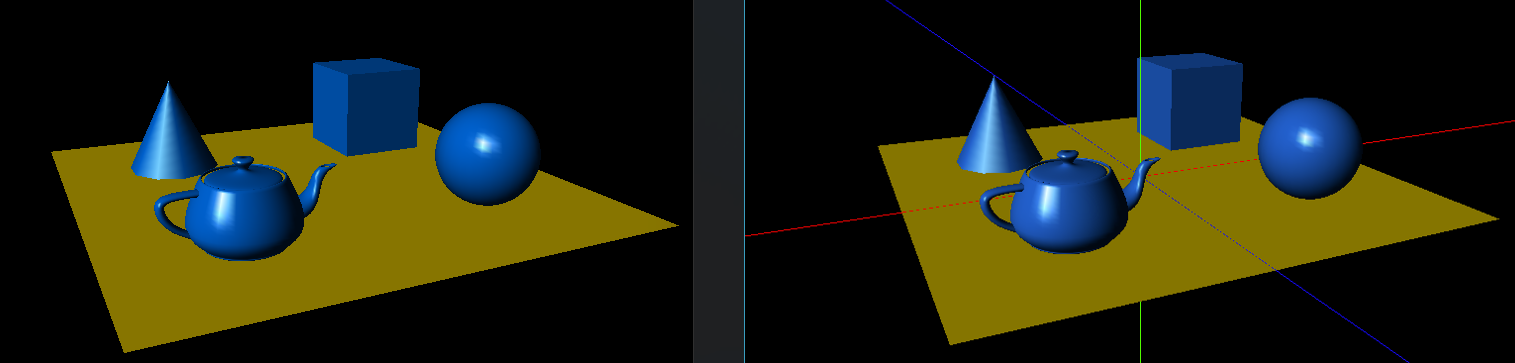
\includegraphics[width=\linewidth]{assets/testes/teste_4_3.png}
            \caption{Resultado do \textit{test_4_3}} \label{fig:teste_4_3}
        \end{figure}
    \end{landscape}

    \begin{landscape}
        \begin{figure}
            \centering
            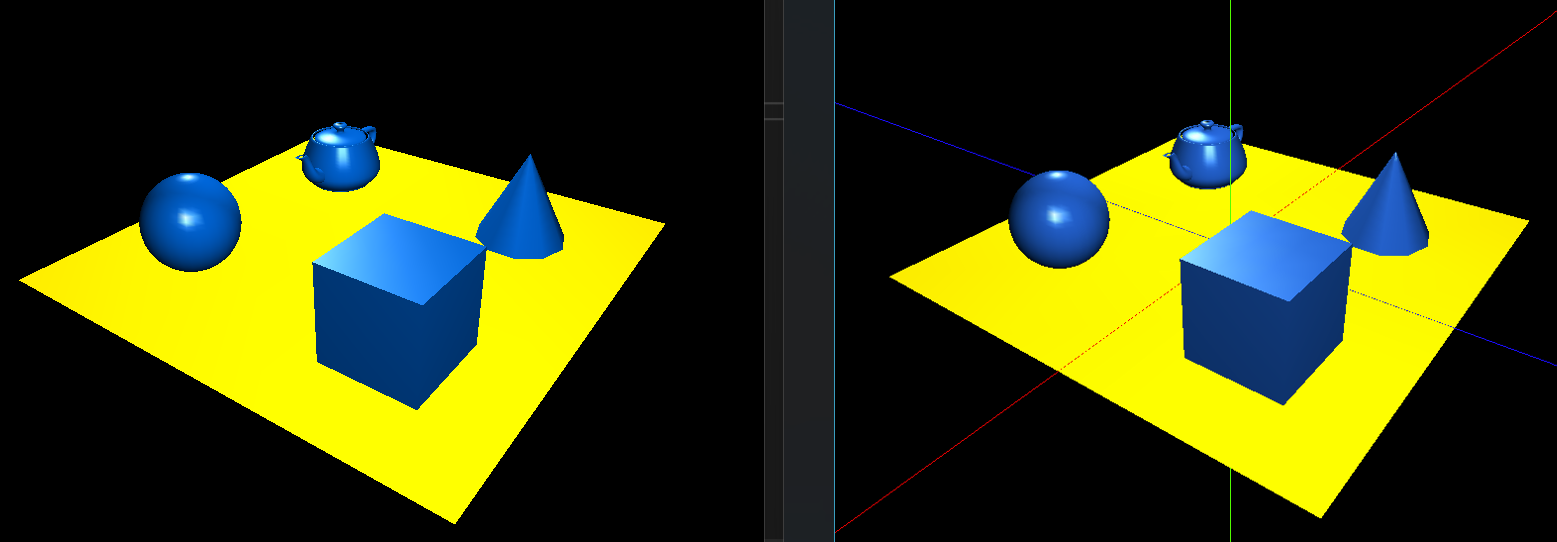
\includegraphics[width=\linewidth]{assets/testes/teste_4_4.png}
            \caption{Resultado do \textit{test_4_4}} \label{fig:teste_4_4}
        \end{figure}
    \end{landscape}

    \begin{landscape}
        \begin{figure}
            \centering
            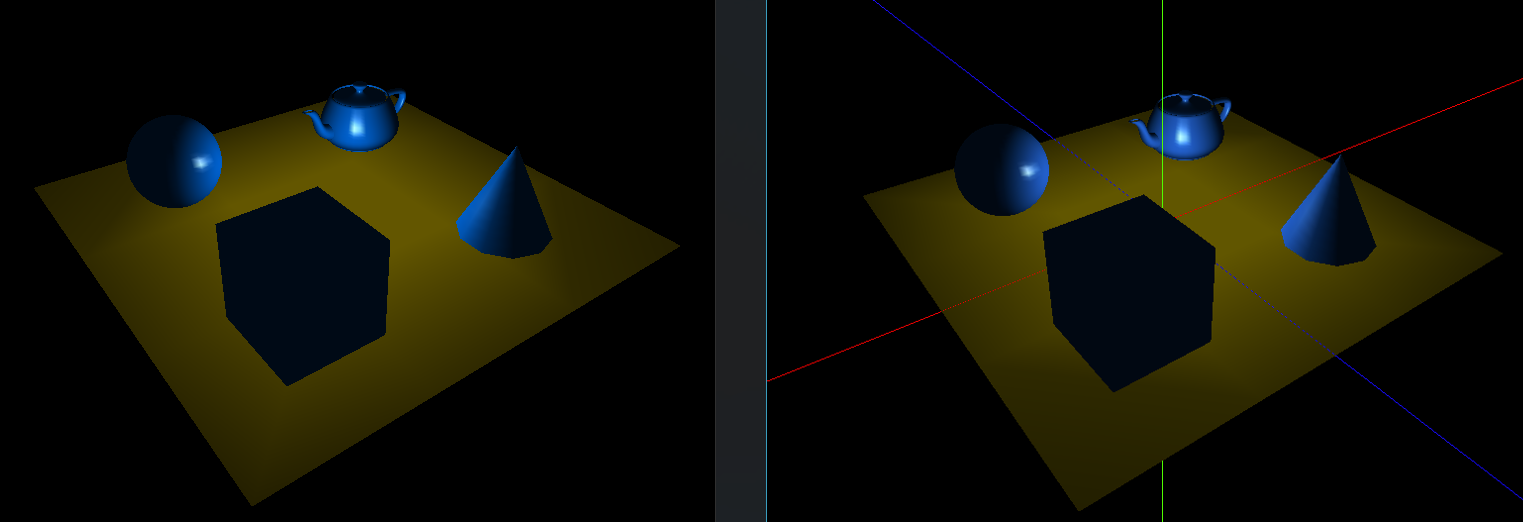
\includegraphics[width=\linewidth]{assets/testes/teste_4_5.png}
            \caption{Resultado do \textit{test_4_5}} \label{fig:teste_4_5}
        \end{figure}
    \end{landscape}

    \begin{landscape}
        \begin{figure}
            \centering
            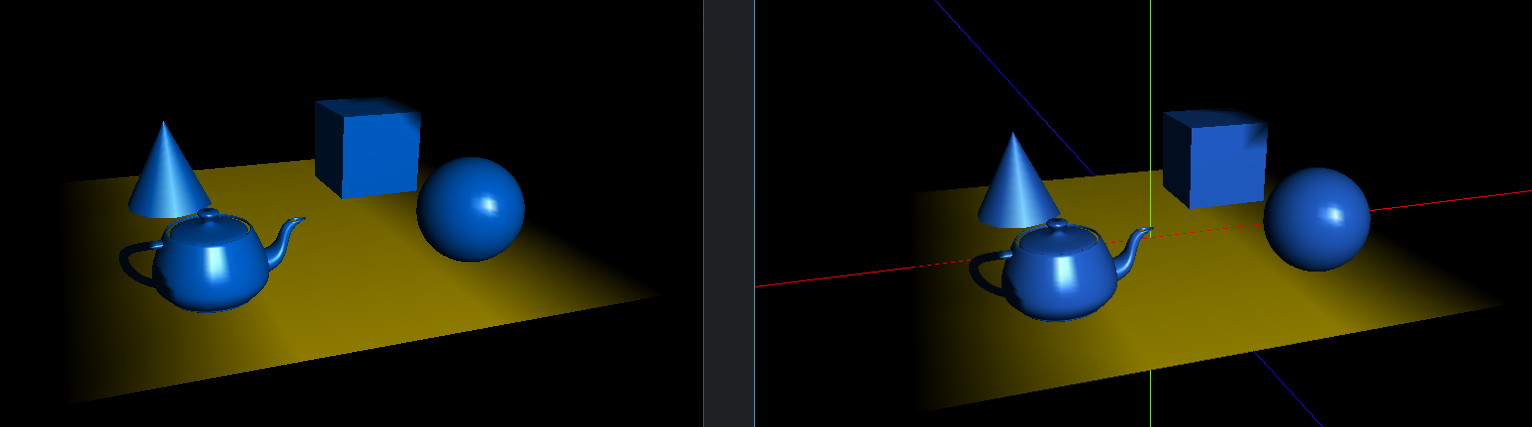
\includegraphics[width=\linewidth]{assets/testes/teste_4_6.png}
            \caption{Resultado do \textit{test_4_6}} \label{fig:teste_4_6}
        \end{figure}
    \end{landscape}

    \begin{landscape}
        \begin{figure}
            \centering
            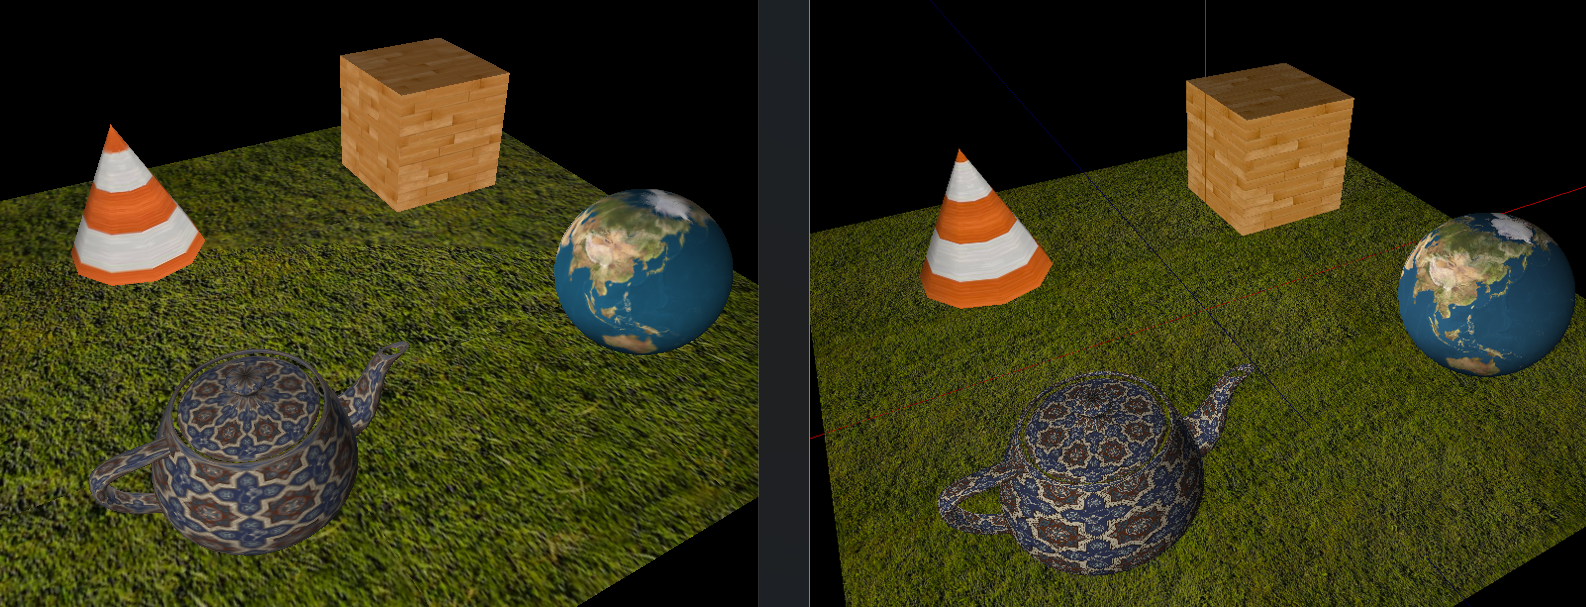
\includegraphics[width=\linewidth]{assets/testes/teste_4_7.png}
            \caption{Resultado do \textit{test_4_7}} \label{fig:teste_4_7}
        \end{figure}
    \end{landscape}

    \subfile{conclusoes.tex}

    \end{document}